\label{sec:overview}

% We proceed to define the testbed environment by each of its conforming
% parts. We later indicate a procedure to set up and configure the testbed
% for several \ac{Raspi}s. In this procedure, we summarize all the key details
% regarding on setting the system files, configuration packages, tools and connectivity
% for the \ac{Raspi}s in a centralized fashion. 

%Afterwards, we indicate how to cross-compile C++ code and the Kodo
%network coding library in an easy way.
%Finally, we provide further information about Kodo itself in terms
%of testing, other platforms supported and source code documentation
%for further references.

%\subsection{System Overview and Design Criteria}

A sketch of the testbed is depicted in Fig.~\ref{fig:testbed_setup}.
The testbed consists of up to 100 \ac{Raspi}s of different models.
More specifically, in our design we consider: Raspberry Pi 1 model B rev.~2,
Raspberry Pi 2 model B V1.1 and Raspberry Pi 3 model B V1.2.
All \ac{Raspi}s are each equipped with a memory card, a wired and wireless
network interface and a power supply. All the \ac{Raspi} are connected to a common
\ac{LAN} that provides internal and external connectivity. Without loss of generality,
in our case they are connected to the university network using their wired Ethernet interface
that is named \texttt{eth0} according to the legacy naming convention of Ethernet
interfaces in Linux~\cite{PredictableNetworkInterfaceNames}. We consider the
university network since we aim the testbed to be used by students and professors
to perform measurements and experimentation of controlled and reproducible scenarios
as part of academic research. We intend to configure all \ac{Raspi}s identically,
while still allowing the end-users to alter how each \ac{Raspi} behaves and is configured.

\begin{figure}[ht!]
\centering
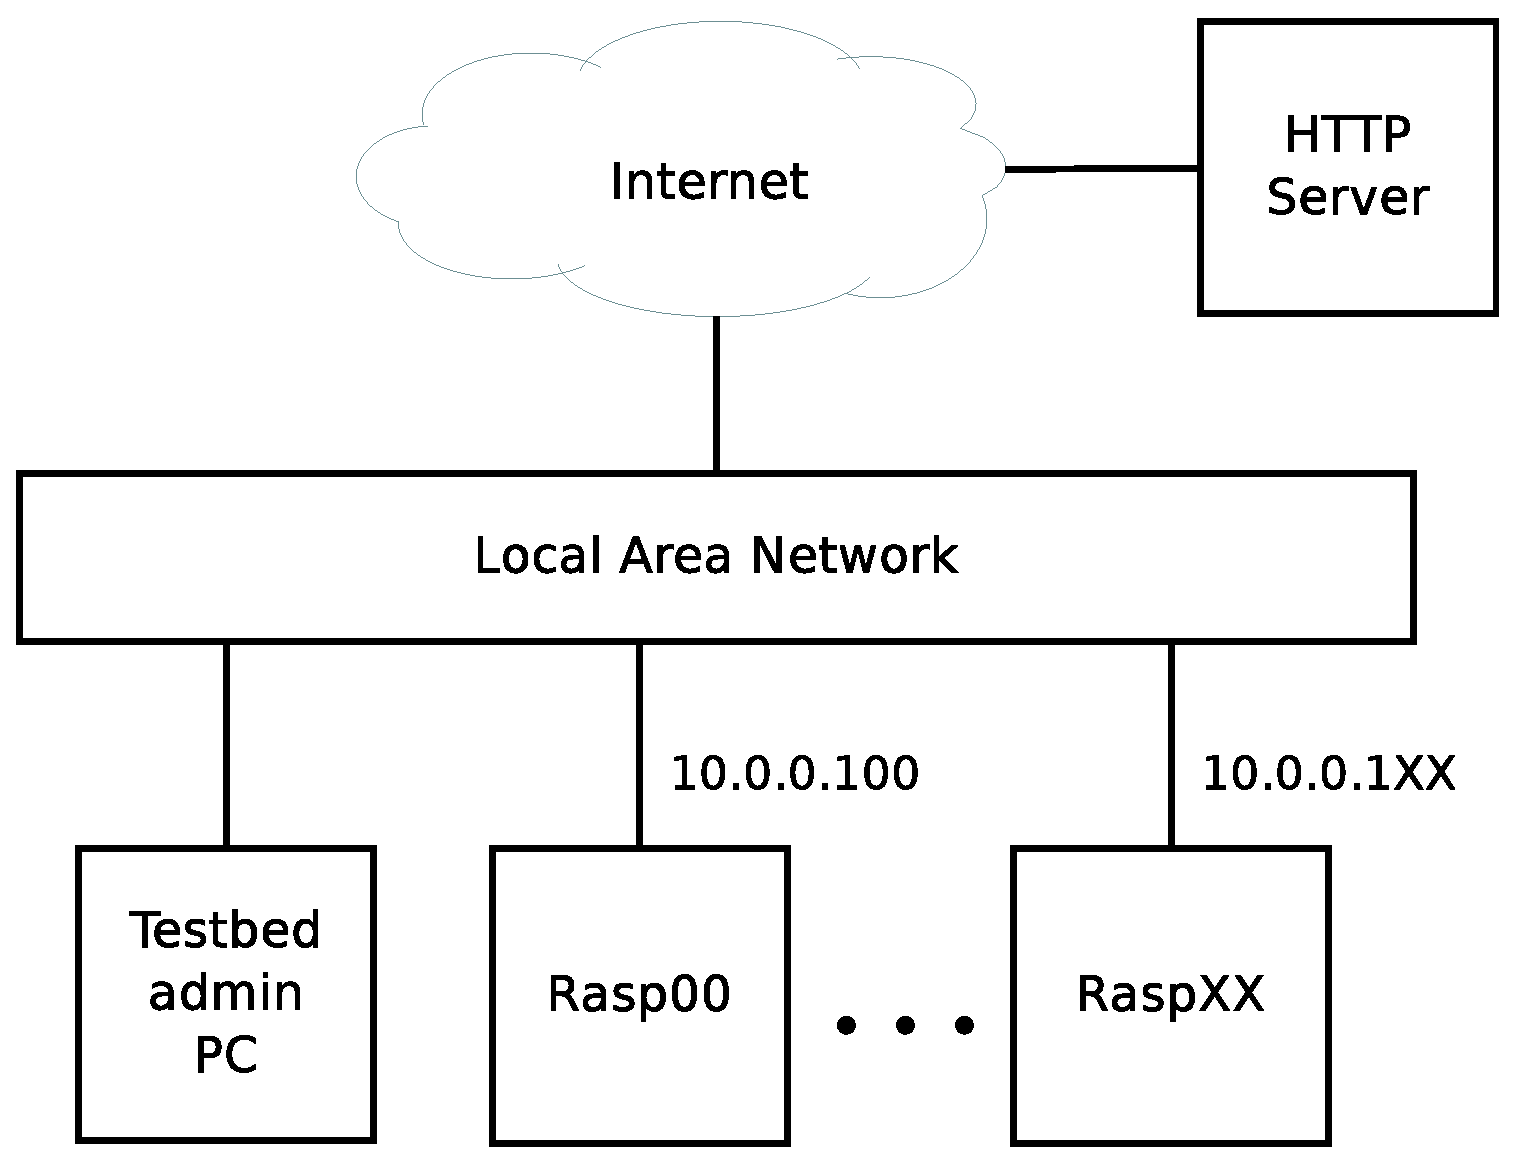
\includegraphics[width=0.45\textwidth]{images/testbed_setup3.eps}
\caption{Testbed setup}
\label{fig:testbed_setup}
\end{figure}

%This significantly eases the management of the \ac{Raspi}s
%as \ac{SSH} eliminates the need for monitors and keyboards for the \ac{Raspi}s.

In Fig.~\ref{fig:testbed_setup} and what follows, we will refer
as the testbed administrator to the person(s) in charge of setting up and configuring
the testbed with administrator privileges from the \ac{OS} point of view.
The setting and configuration procedure commands are performed the testbed administrator in a
regular \ac{PC} running a Linux distribution. Although in principle the administrator
Linux distribution is not a restriction, we present our procedure in a Debian-based Linux
distribution. Finally, our design considers to fetch the \ac{Raspi}s
root filesystem from a \ac{HTTP} server. This enables the testbed administrator to
make filesystem in one location. The \ac{Raspi}s will then get the changes after a reboot.
All \ac{Raspi}s will be configured to run a \ac{SSH} daemon for easy remote access
within the university network. We requested the university \ac{IT} department to
configure the university \ac{DHCP} server to assign each \ac{Raspi} a static
\ac{IP}. This eliminates the requirements of monitors and keyboards with the
\ac{Raspi}s for non-graphical applications.

Based on a regular Raspbian Linux image, we explain how
to customize it to include desired packages for performing routinary tasks and set it
in all the \ac{Raspi}s. Also, when working on a testbed with many devices, it may not always be
desired to make persistent changes to the devices. Thus, we later present how to utilize
stacked filesystems to enable both persistent and temporary
storage. This step of the procedure will be optional if the testbed
administrator decides to write the whole image into a memory card. \todot{Check the
veracity and correctness of the previous statement. Question: Shoudln't we use
an overlay FS regardless of how the memory card is configured?}.
Although being simpler than a stacked filesystem, writing the whole Linux
filesystem to several memory cards may complicate future
maintenance of the testbed since updates need to be performed in each \ac{Raspi}.
Even when tools such as Python Fabric may ease this task, the maintenance might still
be cumbersome in some cases. Therefore, we propose and encourage the alternative centralized
approach where the initial \ac{RAM} filesystem is customized in a way that
enables \ac{Raspi}s to fetch the its root filesystem from a \ac{HTTP} server as
mentioned previously.

%The following procedure explains how the testbed may be setup and configured.

%\textcolor{red}{The testbed should be available for students to perform simulations and
%measurements as part of their semester projects. We intend to configure
%all \ac{Raspi}s identically, while still allowing students to alter
%how each \ac{Raspi} behaves and is configured.
%\\\\
%When working on the testbed with this many devices, it may not always be
%desired to make persistent changes to devices. We present how the concept
%of stacked filesystems may be used to enable the means of both persistent
%and temporary storage.}

%The testbed should be available for students to perform simulations and
%measurements as part of their semester projects. The \ac{Raspi}s should
%be configured identically, but allows the students to alter the
%configurations and how each \ac{Raspi} behaves.
%
%When working on a testbed with many devices, it may not always desired
%to make persistent changes to devices. We present how the concept of stacked
%filesystems may be used to enable the means of both persistent and
%temporary storage.

%A \ac{HTTP} server will be used to store Linux configuration files as well
%as the root filesystem in the centralized approach.

%The following procedure will explain how the testbed may be setup and
%configured both in the traditional distributed fasion where the
%entire Linux filesystem is written to an memory card, but also in a more
%centralized fasion where 
%is written to
%Based on the popular Debian based Raspbian Linux distribution
%We
%first present how a standard Linux distribution for the \ac{Raspi}s
%may be customized 